\documentclass[10pt]{article}\usepackage[margin=.65in]{geometry}\usepackage[T1]{fontenc}\usepackage{graphicx}\setlength{\parindent}{0pt}\setlength{\parskip}{7pt}\sloppy\begin{document}{\large Reviewed genus-2 interface derivations}\par Independent reviews of producer commit 125c631e40 support the written constructions at their stated scope. Fresh native fixed controls support the enumerated examples. No universal Lean chart or complete mutable-state refinement theorem is claimed. No scientific cohort, timing or cost-ratio result was generated; the frozen 1,260-target scope remains intact.\par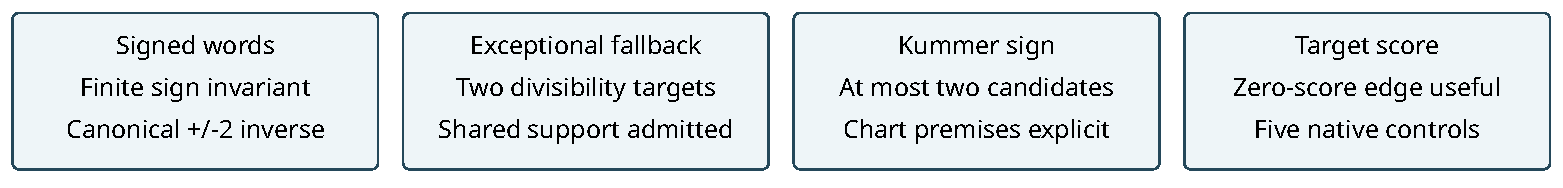
\includegraphics[width=\linewidth]{diagram.pdf}\par Kummer candidate bound. For the ordinary chart, shared u and extracted S=b1 squared leave at most two opposite divisors, including S=0. The argument needs the coordinate correspondence and field premises, but not squarefree support. Neighbour orientation additionally needs its quotient-fiber domain, non-two-torsion anchor, candidate completeness and projection success. Producer 11 and reviewer 7 fixed algebra assertions passed. The review preserves an initial integer-type compilation failure and absent-binary attempt before a corrected fail-closed replay.

Signed words. The finite sign invariant and inverse formulas inverse(+2)=r/2+1 and inverse(-2)=r/2 were checked as written algebra. Canonical narrow addition is bounded for r at most2\textasciicircum{}63. Native callers and invalid-sign behavior were inspected separately; the public graph method does not itself validate the sign predicate. Word-state composition and runtime headroom remain implementation obligations.

Exceptional fallback. The review checked the actual six-register EEA update, common-divisor invariant, normalization and both divisibilities D squared divides UaUb and D divides N. Shared support and Va+Vb=0 remain admitted. The degree-decreasing active-step bound is b.length; a future fuel API must separately define terminal observation. Proposed F17 fixtures were checked by hand algebra, not executed. The next implementation must compose the word EEA endpoint with both native exact divisions.

Target score. Five producer fixture groups and five reviewer fixture groups passed on unchanged native source. Three intentionally inconsistent inputs triggered caught native assertions. A zero-score anchor makes a later edge score 3 and return 6; without it that edge scores 2 and returns no value. Current policy inserts all accepted unseen split edges. First-score-only instrumentation is six scalar-add increments and two find visits, excluding constructor and insertion work. Score totals are not an information metric or a policy comparison.

Review provenance. Producers were published before cross-review, reviewers disclose prior familiarity, and no blind re-derivation is claimed. Written mathematical support, source correspondence and native fixed controls remain separate evidence types. Separate review PDFs, structured statuses, source snapshots, raw outputs and failure records accompany this summary. Compiled build products are omitted from publication while original receipts retain their hashes.
\end{document}